\documentclass{article}
\usepackage[utf8]{inputenc}
\usepackage{graphicx}
\usepackage[margin=1.25in]{geometry}

\setlength{\parindent}{0pt}

\title{CMSC389E - Redstone Basics Guide}
\author{Akilesh Praveen}
\date{}

\begin{document}

\maketitle

\section{Introduction}

Redstone forms the building blocks of logic in Minecraft. Simply put, it is a wiring system within Minecraft that provides players with some very basic logical functions. By leveraging those functions that emulate wiring mechanics in the real world, we can build accurate representations of digital circuits within Minecraft, using redstone.
\newline\newline
If you have taken a digital logic design class already, you may already see some parallels between the components that Redstone provides and components in the real world. However, do not be misled- the functionality of some of these components involve nuances that you may not be aware of.

\section{The Blocks}

When viewing the Creative Mode menu, it's helpful to navigate to the 'Redstone' tab to find what you need for this class very quickly. Although you are provided a multitude of redstone gadgets and tools in this menu, we will only really be using the redstone dust, redstone torch, and redstone repeater items in this class. (Circled in the image below)
\newline

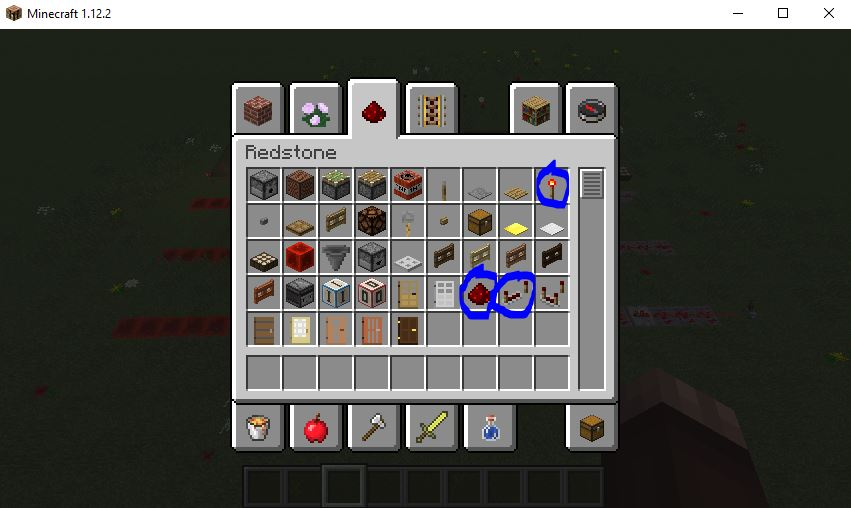
\includegraphics[width=\textwidth]{misc1_1}

\newpage

Using these three items, combined with (most) any block of your choice, it is possible to build a fully programmable computer.

\section{Redstone Current}

Try and place these blocks on the ground of your world in different combinations, and see what happens. As you can imagine, these three components emulate the very basics of wiring in the real world. The redstone wire is analogous to any old piece of copper wire, the redstone torch functions more or less like a source of electricity, and the redstone repeater works as a range extender.
\newline\newline
Thankfully, this is as simple as it gets. In no way will we be using concepts such as Ohm's law or factoring in resistance, current, and voltage- if we did, this would be a circuits class, and I would not be teaching it, as I'm not a sadist.
\newline\newline
Instead, we can see that using redstone to wire up contraptions in Minecraft is fairly trivial. Here are a few key things that you should understand about redstone current.

    \subsection{Redstone wire has two states: On and Off }
    As mentioned above, redstone wiring is a lot more simple than wiring in the real world. It can be in one of two states, on or off. (Or, if you prefer, 1 and 0).\newline
    
    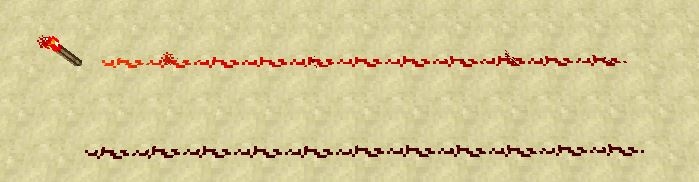
\includegraphics[width=\textwidth]{misc1_2}\newline

    In this image, there are two important points to be noted. First, Redstone torches are a source of an 'on' signal, or as it is colloquially called, 'redstone current'. Second, observe that the vibrance of the red in the 'on' wiring is growing duller the farther from the torch that it gets. This can be somewhat misleading, as one may think that there is a functional difference between more vibrant 'on' wire than duller 'on' wire. In actuality, there is no difference. The reasoning for this feature in Minecraft will be explained below, but for now, take note that wire can only be in one of two states: on or off.
    
    \subsection{Redstone current 'runs out' after 15 blocks }
    Although redstone only has two states as we mentioned, the 'on' state also carries with it a 'current strength'. In other words, if you provide a redstone current to wire using a torch, after 15 blocks worth of redstone wiring, that current will expire. The strength starts at 15, and decreases by 1 for every block that the current traverses, until it finally reaches zero.
    \newline\newline
    Now you might be wondering, why does this happen? It's for a few reasons, some involving limitations of Minecraft itself, among others. Just as an example, if you had a torch at block A, then had a redstone lamp at block B, an infinite amount of blocks from block A, then you'd have the potential to change the state of an infinite amount of wiring instantaneously. As you can imagine, Minecraft's game engine does not enjoy entertaining these possibilities. So, this has been addressed using redstone repeaters.
    
    \subsection{Repeaters provide delay}
    For all intents and purposes, you can think of a redstone repeater as a simple range extender for a redstone current. Remember our previous example with a torch and wire? If we have redstone current flowing through a wire coming from a source 15 blocks away, we can place a repeater down instead of another piece of wire to increase the strength of the current back up to 15. In Vanilla Minecraft, this didn't come for free; redstone repeaters added a small delay in exchange for increasing current strength back up to 15. Additionally, you were able to increase the delay by right clicking on the repeater, if you so desired. You're welcome to read more about repeaters on the Minecraft Wiki if you'd like more information.\newline
    
    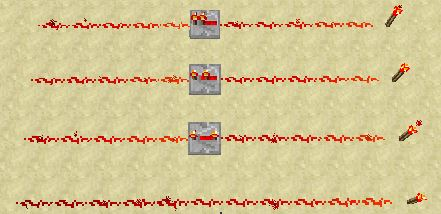
\includegraphics[width=\textwidth]{misc1_3.JPG}\newline
    
    Here, you can see a wiring setup with no repeater (where the current is slowly dying down), a repeater set on the first setting, second, and third setting. As you go from the first to the third setting, you can increase the delay between the inception of the current (in this case, the placing of the torch) and the final piece of wire it is slated to reach. Note that after passing through the repeater, the wire is once again a very vibrant red, signifying that the strength of the current has been once again set to 15.\newline
    
    This allowed circuits to play nice with the game engine. However, we are an adventurous bunch, and we like to live dangerously. For that reason, in the CMSC389E mod, the delay on the first setting of a repeater has been set to 0. As you can imagine, this can be leveraged to wreak havoc on your game engine, but this is also what allows our more complex circuits to function at a pace that isn't agonizingly slow. For that reason, unless you desire a massive delay, we advise you to keep all your repeaters set to the first setting for this class. Not doing so may result in faulty circuits, as you'll see in later projects.
    \newline
    
    \section{Input and Output Blocks}
    
    New in CMSC389E- the input and output blocks are very simple features that allow us to 'test' the circuits that you have made. The idea is this: input blocks will produce a redstone current (identical to how a redstone torch does), and after a set amount of time to accomodate circuit delay, (you can input this when running the test command) the output blocks will expect a certain state, on or off. Note that the strength of the redstone current is irrelevant, and will not be tested.
    \newline\newline
    These blocks are not included in the Vanilla version of Minecraft, so you will only be able to experiment with them in the modded CMSC389E version of the game. You can find more information regarding how to use the input/output blocks on the Project 0 specification document.
    \newline\newline
    As always, feel free to stop by office hours or post a question on Piazza if you have any questions. Now go forth, and experiment!
\end{document}
